% Options for packages loaded elsewhere
\PassOptionsToPackage{unicode}{hyperref}
\PassOptionsToPackage{hyphens}{url}
%
\documentclass[
]{article}
\usepackage{lmodern}
\usepackage{amssymb,amsmath}
\usepackage{ifxetex,ifluatex}
\ifnum 0\ifxetex 1\fi\ifluatex 1\fi=0 % if pdftex
  \usepackage[T1]{fontenc}
  \usepackage[utf8]{inputenc}
  \usepackage{textcomp} % provide euro and other symbols
\else % if luatex or xetex
  \usepackage{unicode-math}
  \defaultfontfeatures{Scale=MatchLowercase}
  \defaultfontfeatures[\rmfamily]{Ligatures=TeX,Scale=1}
\fi
% Use upquote if available, for straight quotes in verbatim environments
\IfFileExists{upquote.sty}{\usepackage{upquote}}{}
\IfFileExists{microtype.sty}{% use microtype if available
  \usepackage[]{microtype}
  \UseMicrotypeSet[protrusion]{basicmath} % disable protrusion for tt fonts
}{}
\makeatletter
\@ifundefined{KOMAClassName}{% if non-KOMA class
  \IfFileExists{parskip.sty}{%
    \usepackage{parskip}
  }{% else
    \setlength{\parindent}{0pt}
    \setlength{\parskip}{6pt plus 2pt minus 1pt}}
}{% if KOMA class
  \KOMAoptions{parskip=half}}
\makeatother
\usepackage{xcolor}
\IfFileExists{xurl.sty}{\usepackage{xurl}}{} % add URL line breaks if available
\IfFileExists{bookmark.sty}{\usepackage{bookmark}}{\usepackage{hyperref}}
\hypersetup{
  pdftitle={Cleaning Data in R},
  pdfauthor={Kim Roth \& Johnathan Clementi},
  hidelinks,
  pdfcreator={LaTeX via pandoc}}
\urlstyle{same} % disable monospaced font for URLs
\usepackage[margin=1in]{geometry}
\usepackage{color}
\usepackage{fancyvrb}
\newcommand{\VerbBar}{|}
\newcommand{\VERB}{\Verb[commandchars=\\\{\}]}
\DefineVerbatimEnvironment{Highlighting}{Verbatim}{commandchars=\\\{\}}
% Add ',fontsize=\small' for more characters per line
\usepackage{framed}
\definecolor{shadecolor}{RGB}{248,248,248}
\newenvironment{Shaded}{\begin{snugshade}}{\end{snugshade}}
\newcommand{\AlertTok}[1]{\textcolor[rgb]{0.94,0.16,0.16}{#1}}
\newcommand{\AnnotationTok}[1]{\textcolor[rgb]{0.56,0.35,0.01}{\textbf{\textit{#1}}}}
\newcommand{\AttributeTok}[1]{\textcolor[rgb]{0.77,0.63,0.00}{#1}}
\newcommand{\BaseNTok}[1]{\textcolor[rgb]{0.00,0.00,0.81}{#1}}
\newcommand{\BuiltInTok}[1]{#1}
\newcommand{\CharTok}[1]{\textcolor[rgb]{0.31,0.60,0.02}{#1}}
\newcommand{\CommentTok}[1]{\textcolor[rgb]{0.56,0.35,0.01}{\textit{#1}}}
\newcommand{\CommentVarTok}[1]{\textcolor[rgb]{0.56,0.35,0.01}{\textbf{\textit{#1}}}}
\newcommand{\ConstantTok}[1]{\textcolor[rgb]{0.00,0.00,0.00}{#1}}
\newcommand{\ControlFlowTok}[1]{\textcolor[rgb]{0.13,0.29,0.53}{\textbf{#1}}}
\newcommand{\DataTypeTok}[1]{\textcolor[rgb]{0.13,0.29,0.53}{#1}}
\newcommand{\DecValTok}[1]{\textcolor[rgb]{0.00,0.00,0.81}{#1}}
\newcommand{\DocumentationTok}[1]{\textcolor[rgb]{0.56,0.35,0.01}{\textbf{\textit{#1}}}}
\newcommand{\ErrorTok}[1]{\textcolor[rgb]{0.64,0.00,0.00}{\textbf{#1}}}
\newcommand{\ExtensionTok}[1]{#1}
\newcommand{\FloatTok}[1]{\textcolor[rgb]{0.00,0.00,0.81}{#1}}
\newcommand{\FunctionTok}[1]{\textcolor[rgb]{0.00,0.00,0.00}{#1}}
\newcommand{\ImportTok}[1]{#1}
\newcommand{\InformationTok}[1]{\textcolor[rgb]{0.56,0.35,0.01}{\textbf{\textit{#1}}}}
\newcommand{\KeywordTok}[1]{\textcolor[rgb]{0.13,0.29,0.53}{\textbf{#1}}}
\newcommand{\NormalTok}[1]{#1}
\newcommand{\OperatorTok}[1]{\textcolor[rgb]{0.81,0.36,0.00}{\textbf{#1}}}
\newcommand{\OtherTok}[1]{\textcolor[rgb]{0.56,0.35,0.01}{#1}}
\newcommand{\PreprocessorTok}[1]{\textcolor[rgb]{0.56,0.35,0.01}{\textit{#1}}}
\newcommand{\RegionMarkerTok}[1]{#1}
\newcommand{\SpecialCharTok}[1]{\textcolor[rgb]{0.00,0.00,0.00}{#1}}
\newcommand{\SpecialStringTok}[1]{\textcolor[rgb]{0.31,0.60,0.02}{#1}}
\newcommand{\StringTok}[1]{\textcolor[rgb]{0.31,0.60,0.02}{#1}}
\newcommand{\VariableTok}[1]{\textcolor[rgb]{0.00,0.00,0.00}{#1}}
\newcommand{\VerbatimStringTok}[1]{\textcolor[rgb]{0.31,0.60,0.02}{#1}}
\newcommand{\WarningTok}[1]{\textcolor[rgb]{0.56,0.35,0.01}{\textbf{\textit{#1}}}}
\usepackage{graphicx,grffile}
\makeatletter
\def\maxwidth{\ifdim\Gin@nat@width>\linewidth\linewidth\else\Gin@nat@width\fi}
\def\maxheight{\ifdim\Gin@nat@height>\textheight\textheight\else\Gin@nat@height\fi}
\makeatother
% Scale images if necessary, so that they will not overflow the page
% margins by default, and it is still possible to overwrite the defaults
% using explicit options in \includegraphics[width, height, ...]{}
\setkeys{Gin}{width=\maxwidth,height=\maxheight,keepaspectratio}
% Set default figure placement to htbp
\makeatletter
\def\fps@figure{htbp}
\makeatother
\setlength{\emergencystretch}{3em} % prevent overfull lines
\providecommand{\tightlist}{%
  \setlength{\itemsep}{0pt}\setlength{\parskip}{0pt}}
\setcounter{secnumdepth}{-\maxdimen} % remove section numbering

\title{Cleaning Data in R}
\author{Kim Roth \& Johnathan Clementi}
\date{3/3/2020}

\begin{document}
\maketitle

Library load

\begin{Shaded}
\begin{Highlighting}[]
\KeywordTok{library}\NormalTok{(tidyverse) }\CommentTok{#loads ggplot and the others}
\KeywordTok{library}\NormalTok{(readxl)}\CommentTok{#for reading in excel files}
\end{Highlighting}
\end{Shaded}

The advantage of cleaning data in R rather than excel is that you have a
replicable process should you ever wonder what you did when cleaning or
need to change it.

Most important tip when cleaning. Always keep the original data file.
Always. This is fortunately the default in R.

In case you need a reminder. The data set is data from JC Blair Hospital
based on data they collect yearly at the Huntingdon County Fair about
blood pressure and demographics from voluntary participation by fair
attendees.

Upload the data file from moodle and then use File-\textgreater Import
Data Set-\textgreater{} from Excel. You'll need to change my code for
this to work.

\begin{Shaded}
\begin{Highlighting}[]
\NormalTok{Pressure <-}\StringTok{ }\KeywordTok{read_excel}\NormalTok{(}\StringTok{"C:/Users/clemenj/Google Drive/Grad School/Juniata_DataScience/DS500/Week6/Bloodpressuredata.xlsx"}\NormalTok{)}
\end{Highlighting}
\end{Shaded}

\begin{verbatim}
## Warning in read_fun(path = enc2native(normalizePath(path)), sheet_i = sheet, :
## Expecting numeric in L2985 / R2985C12: got '62"'
\end{verbatim}

\begin{verbatim}
## Warning in read_fun(path = enc2native(normalizePath(path)), sheet_i = sheet, :
## Expecting numeric in L3039 / R3039C12: got '56"'
\end{verbatim}

\begin{verbatim}
## Warning in read_fun(path = enc2native(normalizePath(path)), sheet_i = sheet, :
## Expecting numeric in I3553 / R3553C9: got 'Too old'
\end{verbatim}

Variables: OVERALL-a number assoiated with the case, essentially a case
ID YEAR-What year was the data taked REC- a number associated with case
and year. Essentially which entry was this for this year. BP-blood
pressure as a ratio, systolic/diastolic BP Ratio-The blood pressure
ratio converted to a decimal Systolic-The top number in blood pressure
Diastolic-The bottom number in blood pressure. BP Status-Whether the
blood pressure is Low, Normal, Pre-Hypertension, Hypertension
Age-reported age of person survey Weight- measured weight of person in
pounds Height- height measured in feet and inches Height-Inches-height
measured in inches BMI-a ratio of sorts between height and weight BMI
Category-a category based on BMI Gender-reported gender of participant
Diagnosed Diabetic-report of the participant if ever diagnosed diabetic
Tobacco User-report of the participant if they use tobacco
OnmedicationforBP-report of the participant if they are on medication
for high blood pressure HuntingdonCountyResident-is the participant a
resident of Huntingdon County Date-Date data taken

\begin{Shaded}
\begin{Highlighting}[]
\KeywordTok{str}\NormalTok{(Pressure) }\CommentTok{#view variables and types}
\end{Highlighting}
\end{Shaded}

\begin{verbatim}
## Classes 'tbl_df', 'tbl' and 'data.frame':    3670 obs. of  20 variables:
##  $ OVERALL                 : num  1 2 3 4 5 6 7 8 9 10 ...
##  $ YEAR                    : num  2007 2007 2007 2007 2007 ...
##  $ REC                     : num  1 2 3 4 5 6 7 8 9 10 ...
##  $ BP                      : chr  "147/84" "133/78" "143/89" "156/68" ...
##  $ BP Ratio                : num  1.75 1.71 1.61 2.29 1.6 ...
##  $ Systolic                : num  147 133 143 156 147 130 122 148 152 138 ...
##  $ Diastolic               : num  84 78 89 68 92 88 65 78 86 49 ...
##  $ BP Status               : chr  "Hypertension" "Pre-Hypertension" "Hypertension" "Hypertension" ...
##  $ Age                     : num  51 49 NA NA NA NA NA 74 48 78 ...
##  $ Weight                  : num  201 155 NA NA NA NA NA 206 185 125 ...
##  $ Height                  : chr  NA NA NA NA ...
##  $ Height-Inches           : num  74 70 NA NA NA NA NA 64 64 64 ...
##  $ BMI                     : num  25.8 22.2 NA NA NA ...
##  $ BMI Category            : chr  "Overweight" "Normal" NA NA ...
##  $ Gender                  : chr  "M" "M" "N/A" "N/A" ...
##  $ DiagnosedDiabetic       : chr  "N" "N" "N/A" "N/A" ...
##  $ TobaccoUser             : chr  "N" "Y" "N/A" "N/A" ...
##  $ OnmedicationforBP       : chr  "N" "N" "N/A" "N/A" ...
##  $ HuntingdonCountyResident: chr  "Y" "Y" "N/A" "N/A" ...
##  $ Date                    : chr  NA NA NA NA ...
\end{verbatim}

\begin{enumerate}
\def\labelenumi{\arabic{enumi}.}
\tightlist
\item
  Which variable names have spaces or extra characters like -? 1A.
  \texttt{BP\ Ratio}, \texttt{BP\ Status}, \texttt{Height-Inches},
  \texttt{BMI\ Category}
\end{enumerate}

We would prefer that the names of variables not have spaces (R can be
obnoxious about that)

Here is how to fix BP Status, to make the name ``BPStatus''. Using the
pipe \texttt{\%\textgreater{}\%} is not required, but we will practice
using the pipe throughout this file.

\begin{Shaded}
\begin{Highlighting}[]
\NormalTok{Pressure=Pressure }\OperatorTok\StringTok{ }
\StringTok{  }\KeywordTok{rename}\NormalTok{( }\DataTypeTok{BPStatus=}\StringTok{`}\DataTypeTok{BP Status}\StringTok{`}\NormalTok{) }\CommentTok{#renames the variable. Note the use of the pipe}
\KeywordTok{str}\NormalTok{(Pressure) }\CommentTok{#checking results}
\end{Highlighting}
\end{Shaded}

\begin{verbatim}
## Classes 'tbl_df', 'tbl' and 'data.frame':    3670 obs. of  20 variables:
##  $ OVERALL                 : num  1 2 3 4 5 6 7 8 9 10 ...
##  $ YEAR                    : num  2007 2007 2007 2007 2007 ...
##  $ REC                     : num  1 2 3 4 5 6 7 8 9 10 ...
##  $ BP                      : chr  "147/84" "133/78" "143/89" "156/68" ...
##  $ BP Ratio                : num  1.75 1.71 1.61 2.29 1.6 ...
##  $ Systolic                : num  147 133 143 156 147 130 122 148 152 138 ...
##  $ Diastolic               : num  84 78 89 68 92 88 65 78 86 49 ...
##  $ BPStatus                : chr  "Hypertension" "Pre-Hypertension" "Hypertension" "Hypertension" ...
##  $ Age                     : num  51 49 NA NA NA NA NA 74 48 78 ...
##  $ Weight                  : num  201 155 NA NA NA NA NA 206 185 125 ...
##  $ Height                  : chr  NA NA NA NA ...
##  $ Height-Inches           : num  74 70 NA NA NA NA NA 64 64 64 ...
##  $ BMI                     : num  25.8 22.2 NA NA NA ...
##  $ BMI Category            : chr  "Overweight" "Normal" NA NA ...
##  $ Gender                  : chr  "M" "M" "N/A" "N/A" ...
##  $ DiagnosedDiabetic       : chr  "N" "N" "N/A" "N/A" ...
##  $ TobaccoUser             : chr  "N" "Y" "N/A" "N/A" ...
##  $ OnmedicationforBP       : chr  "N" "N" "N/A" "N/A" ...
##  $ HuntingdonCountyResident: chr  "Y" "Y" "N/A" "N/A" ...
##  $ Date                    : chr  NA NA NA NA ...
\end{verbatim}

\begin{enumerate}
\def\labelenumi{\arabic{enumi}.}
\setcounter{enumi}{1}
\item
  What happens if we rerun the above code again for the second time?
  Why? 2A. The code looks for \texttt{BP\ Status}, however the variable
  name \texttt{BP\ Status} no longer exists in the dataframe because it
  was changed to \texttt{BPStatus}.
\item
  You do the same for any other variables that have spaces in the names.
  Make sure to use the pipe whereever possible. 3A.
\end{enumerate}

\begin{Shaded}
\begin{Highlighting}[]
\NormalTok{Pressure =}\StringTok{ }\NormalTok{Pressure }\OperatorTok
\StringTok{  }\KeywordTok{rename}\NormalTok{(}\DataTypeTok{BPRatio =} \StringTok{`}\DataTypeTok{BP Ratio}\StringTok{`}\NormalTok{, }\DataTypeTok{HeightInches =} \StringTok{`}\DataTypeTok{Height-Inches}\StringTok{`}\NormalTok{, }\DataTypeTok{BMICat =} \StringTok{`}\DataTypeTok{BMI Category}\StringTok{`}\NormalTok{)}
\KeywordTok{str}\NormalTok{(Pressure)}
\end{Highlighting}
\end{Shaded}

\begin{verbatim}
## Classes 'tbl_df', 'tbl' and 'data.frame':    3670 obs. of  20 variables:
##  $ OVERALL                 : num  1 2 3 4 5 6 7 8 9 10 ...
##  $ YEAR                    : num  2007 2007 2007 2007 2007 ...
##  $ REC                     : num  1 2 3 4 5 6 7 8 9 10 ...
##  $ BP                      : chr  "147/84" "133/78" "143/89" "156/68" ...
##  $ BPRatio                 : num  1.75 1.71 1.61 2.29 1.6 ...
##  $ Systolic                : num  147 133 143 156 147 130 122 148 152 138 ...
##  $ Diastolic               : num  84 78 89 68 92 88 65 78 86 49 ...
##  $ BPStatus                : chr  "Hypertension" "Pre-Hypertension" "Hypertension" "Hypertension" ...
##  $ Age                     : num  51 49 NA NA NA NA NA 74 48 78 ...
##  $ Weight                  : num  201 155 NA NA NA NA NA 206 185 125 ...
##  $ Height                  : chr  NA NA NA NA ...
##  $ HeightInches            : num  74 70 NA NA NA NA NA 64 64 64 ...
##  $ BMI                     : num  25.8 22.2 NA NA NA ...
##  $ BMICat                  : chr  "Overweight" "Normal" NA NA ...
##  $ Gender                  : chr  "M" "M" "N/A" "N/A" ...
##  $ DiagnosedDiabetic       : chr  "N" "N" "N/A" "N/A" ...
##  $ TobaccoUser             : chr  "N" "Y" "N/A" "N/A" ...
##  $ OnmedicationforBP       : chr  "N" "N" "N/A" "N/A" ...
##  $ HuntingdonCountyResident: chr  "Y" "Y" "N/A" "N/A" ...
##  $ Date                    : chr  NA NA NA NA ...
\end{verbatim}

\begin{enumerate}
\def\labelenumi{\arabic{enumi}.}
\setcounter{enumi}{3}
\tightlist
\item
  Use select to remove the variable Height. 4A.
\end{enumerate}

\begin{Shaded}
\begin{Highlighting}[]
\NormalTok{Pressure =}\StringTok{ }\KeywordTok{select}\NormalTok{(Pressure, }\OperatorTok{-}\NormalTok{Height)}
\end{Highlighting}
\end{Shaded}

Now let's consider one problem we found last time with Gender. For
reference ggplot does not use pipe without using the ggpipe package.

\begin{Shaded}
\begin{Highlighting}[]
\KeywordTok{ggplot}\NormalTok{(Pressure)}\OperatorTok{+}\KeywordTok{geom_bar}\NormalTok{(}\KeywordTok{aes}\NormalTok{(}\DataTypeTok{x=}\NormalTok{Gender))}
\end{Highlighting}
\end{Shaded}

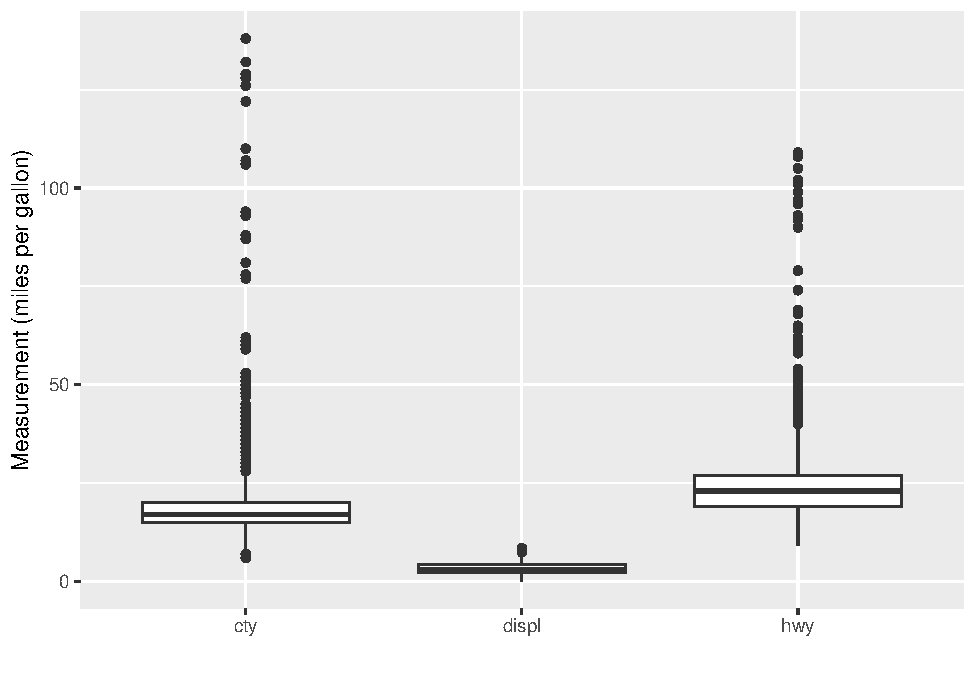
\includegraphics{ClementiHospitalDataCleaning_files/figure-latex/unnamed-chunk-7-1.pdf}

\begin{Shaded}
\begin{Highlighting}[]
\NormalTok{Pressure }\OperatorTok
\KeywordTok{count}\NormalTok{(Gender)}
\end{Highlighting}
\end{Shaded}

\begin{verbatim}
## # A tibble: 6 x 2
##   Gender     n
##   <chr>  <int>
## 1 f          1
## 2 F       1787
## 3 M       1337
## 4 N          1
## 5 N/A      370
## 6 <NA>     174
\end{verbatim}

Now we can see some problems.

\begin{enumerate}
\def\labelenumi{\alph{enumi})}
\item
  f should be F
\item
  N should be M (they are next to each other on the keyboard, it's a
  common typo)
\item
  N/A should be NA.
\end{enumerate}

Here is one way to fix them, we will use the command ifelse along with
mutate. The command works like ifelse(condition to test, what to do if
true, what to do if false)

\begin{Shaded}
\begin{Highlighting}[]
\NormalTok{Pressure=Pressure }\OperatorTok\StringTok{ }
\StringTok{  }\KeywordTok{mutate}\NormalTok{( }\DataTypeTok{Gender=}\KeywordTok{ifelse}\NormalTok{(Gender}\OperatorTok{==}\StringTok{"f"}\NormalTok{, }\StringTok{"F"}\NormalTok{, Gender)) }\CommentTok{#fixing the f to F}
\NormalTok{Pressure }\OperatorTok
\StringTok{  }\KeywordTok{count}\NormalTok{(Gender) }\CommentTok{#checking}
\end{Highlighting}
\end{Shaded}

\begin{verbatim}
## # A tibble: 5 x 2
##   Gender     n
##   <chr>  <int>
## 1 F       1788
## 2 M       1337
## 3 N          1
## 4 N/A      370
## 5 <NA>     174
\end{verbatim}

You can nest the commands too if you want to fix more than one. You can
also fix more than one variable at a time. Here is fixing the N and the
N/A problem together.

\begin{Shaded}
\begin{Highlighting}[]
\NormalTok{Pressure=}
\StringTok{  }\NormalTok{Pressure}\OperatorTok
\StringTok{  }\KeywordTok{mutate}\NormalTok{(}\DataTypeTok{Gender=}\KeywordTok{ifelse}\NormalTok{(Gender}\OperatorTok{==}\StringTok{"N"}\NormalTok{, }\StringTok{"M"}\NormalTok{, }\KeywordTok{ifelse}\NormalTok{(Gender}\OperatorTok{==}\StringTok{"N/A"}\NormalTok{, }\OtherTok{NA}\NormalTok{, Gender))) }
\NormalTok{Pressure}\OperatorTok
\KeywordTok{count}\NormalTok{( Gender) }\CommentTok{#checking}
\end{Highlighting}
\end{Shaded}

\begin{verbatim}
## # A tibble: 3 x 2
##   Gender     n
##   <chr>  <int>
## 1 F       1788
## 2 M       1338
## 3 <NA>     544
\end{verbatim}

\begin{enumerate}
\def\labelenumi{\arabic{enumi}.}
\setcounter{enumi}{4}
\tightlist
\item
  Pick another categorical variable (I believe they all have something
  wrong, often multiple somethings). Examine the variable and then fix
  the problem(s). Use pipe whenever possible. 5A.
\end{enumerate}

\begin{Shaded}
\begin{Highlighting}[]
\KeywordTok{count}\NormalTok{(Pressure, TobaccoUser)}
\end{Highlighting}
\end{Shaded}

\begin{verbatim}
## # A tibble: 5 x 2
##   TobaccoUser     n
##   <chr>       <int>
## 1 M               1
## 2 N            3001
## 3 N/A            63
## 4 Y             594
## 5 <NA>           11
\end{verbatim}

\begin{Shaded}
\begin{Highlighting}[]
\NormalTok{Pressure =}
\StringTok{  }\NormalTok{Pressure }\OperatorTok
\StringTok{  }\KeywordTok{mutate}\NormalTok{(}\DataTypeTok{TobaccoUser=}\KeywordTok{ifelse}\NormalTok{(TobaccoUser}\OperatorTok{==}\StringTok{"M"}\NormalTok{, }\StringTok{"N"}\NormalTok{, }\KeywordTok{ifelse}\NormalTok{(TobaccoUser}\OperatorTok{==}\StringTok{"N/A"}\NormalTok{, }\OtherTok{NA}\NormalTok{, TobaccoUser)))}
\NormalTok{Pressure}\OperatorTok
\KeywordTok{count}\NormalTok{(TobaccoUser)}
\end{Highlighting}
\end{Shaded}

\begin{verbatim}
## # A tibble: 3 x 2
##   TobaccoUser     n
##   <chr>       <int>
## 1 N            3002
## 2 Y             594
## 3 <NA>           74
\end{verbatim}

Now that we know summarize, we will use it to summarize variables.

\begin{Shaded}
\begin{Highlighting}[]
\NormalTok{Pressure }\OperatorTok
\KeywordTok{summarize}\NormalTok{(}\DataTypeTok{MaxSys=}\KeywordTok{max}\NormalTok{(Systolic, }\DataTypeTok{na.rm=}\OtherTok{TRUE}\NormalTok{), }\DataTypeTok{MinSys=}\KeywordTok{min}\NormalTok{(Systolic, }\DataTypeTok{na.rm=}\OtherTok{TRUE}\NormalTok{), }\DataTypeTok{MeanSys=}\KeywordTok{mean}\NormalTok{(Systolic, }\DataTypeTok{na.rm=}\OtherTok{TRUE}\NormalTok{))}
\end{Highlighting}
\end{Shaded}

\begin{verbatim}
## # A tibble: 1 x 3
##   MaxSys MinSys MeanSys
##    <dbl>  <dbl>   <dbl>
## 1    814      0    130.
\end{verbatim}

We will want to identify how many readings are unreasonable. For now, we
will assume the systolic blood pressure reading is in a range where it
wouldn't send a person to the hospital. That is between 80 (based on
\url{https://www.mayoclinic.org/diseases-conditions/low-blood-pressure/symptoms-causes/syc-20355465})
and 190 (based on
\url{https://www.heart.org/en/health-topics/high-blood-pressure/understanding-blood-pressure-readings})
using 10 as a margin of error. Normally we would ask the client what
levels they'd want removed.

Here are the too high and too low ones. It is often worth looking at the
outliers.

\begin{Shaded}
\begin{Highlighting}[]
\NormalTok{Pressure }\OperatorTok
\KeywordTok{filter}\NormalTok{( Systolic}\OperatorTok{>}\DecValTok{190}\OperatorTok{|}\NormalTok{Systolic}\OperatorTok{<}\DecValTok{80}\NormalTok{)}
\end{Highlighting}
\end{Shaded}

\begin{verbatim}
## # A tibble: 24 x 19
##    OVERALL  YEAR   REC BP    BPRatio Systolic Diastolic BPStatus   Age Weight
##      <dbl> <dbl> <dbl> <chr>   <dbl>    <dbl>     <dbl> <chr>    <dbl>  <dbl>
##  1      25  2007    25 201/~    1.58      201       127 Hyperte~    56     NA
##  2     501  2007   501 192/~    2.29      192        84 Hyperte~    86    160
##  3     563  2007   563 193/~    2.44      193        79 Hyperte~    63    210
##  4     662  2009    22 79/41    1.93       79        41 Optimal     69    302
##  5     686  2009    46 191/~    2.17      191        88 Hyperte~    61    185
##  6     840  2009   200 72/46    1.57       72        46 Optimal     59    177
##  7     990  2009   350 211/~    2.24      211        94 Hyperte~    50     NA
##  8    1091  2009   451 198/~    2.28      198        87 Hyperte~    66    187
##  9    1176  2009   536 78/61    1.28       78        61 Optimal     48    248
## 10    1194  2009   554 70/47    1.49       70        47 Optimal     62    140
## # ... with 14 more rows, and 9 more variables: HeightInches <dbl>, BMI <dbl>,
## #   BMICat <chr>, Gender <chr>, DiagnosedDiabetic <chr>, TobaccoUser <chr>,
## #   OnmedicationforBP <chr>, HuntingdonCountyResident <chr>, Date <chr>
\end{verbatim}

Here is an alternate method for looking too high or too low using
arrange

\begin{Shaded}
\begin{Highlighting}[]
\NormalTok{Pressure }\OperatorTok\StringTok{ }
\StringTok{  }\KeywordTok{arrange}\NormalTok{(Systolic)}
\end{Highlighting}
\end{Shaded}

\begin{verbatim}
## # A tibble: 3,670 x 19
##    OVERALL  YEAR   REC BP    BPRatio Systolic Diastolic BPStatus   Age Weight
##      <dbl> <dbl> <dbl> <chr>   <dbl>    <dbl>     <dbl> <chr>    <dbl>  <dbl>
##  1    2703  2012   150 000/~   NA           0         0 Optimal     72    126
##  2    2780  2012   227 000/~   NA           0         0 Optimal     46    190
##  3    2813  2012   260 000/~   NA           0         0 Optimal     58    130
##  4    2887  2012   334 000/~   NA           0         0 Optimal     84    195
##  5    4021  2012   467 000/~   NA           0         0 Optimal     68    185
##  6    4089  2012   535 000/~   NA           0         0 Optimal     70    190
##  7    4090  2012   536 000/~   NA           0         0 Optimal     57    145
##  8    1194  2009   554 70/47    1.49       70        47 Optimal     62    140
##  9     840  2009   200 72/46    1.57       72        46 Optimal     59    177
## 10    1176  2009   536 78/61    1.28       78        61 Optimal     48    248
## # ... with 3,660 more rows, and 9 more variables: HeightInches <dbl>,
## #   BMI <dbl>, BMICat <chr>, Gender <chr>, DiagnosedDiabetic <chr>,
## #   TobaccoUser <chr>, OnmedicationforBP <chr>, HuntingdonCountyResident <chr>,
## #   Date <chr>
\end{verbatim}

\begin{Shaded}
\begin{Highlighting}[]
\NormalTok{Pressure }\OperatorTok\StringTok{ }
\StringTok{  }\KeywordTok{arrange}\NormalTok{(}\KeywordTok{desc}\NormalTok{(Systolic))}
\end{Highlighting}
\end{Shaded}

\begin{verbatim}
## # A tibble: 3,670 x 19
##    OVERALL  YEAR   REC BP    BPRatio Systolic Diastolic BPStatus   Age Weight
##      <dbl> <dbl> <dbl> <chr>   <dbl>    <dbl>     <dbl> <chr>    <dbl>  <dbl>
##  1    1636  2010   413 814/~    9.47      814        86 Hyperte~    72    223
##  2     990  2009   350 211/~    2.24      211        94 Hyperte~    50     NA
##  3    1595  2010   372 208/~    2.21      208        94 Hyperte~    52    350
##  4    1283  2010    60 206/~    1.79      206       115 Hyperte~    59    214
##  5      25  2007    25 201/~    1.58      201       127 Hyperte~    56     NA
##  6    1091  2009   451 198/~    2.28      198        87 Hyperte~    66    187
##  7    1750  2010   527 198/~    1.98      198       100 Hyperte~    43    230
##  8     563  2007   563 193/~    2.44      193        79 Hyperte~    63    210
##  9    4085  2013   294 193/~    3.11      193        62 <NA>        88    159
## 10     501  2007   501 192/~    2.29      192        84 Hyperte~    86    160
## # ... with 3,660 more rows, and 9 more variables: HeightInches <dbl>,
## #   BMI <dbl>, BMICat <chr>, Gender <chr>, DiagnosedDiabetic <chr>,
## #   TobaccoUser <chr>, OnmedicationforBP <chr>, HuntingdonCountyResident <chr>,
## #   Date <chr>
\end{verbatim}

\begin{enumerate}
\def\labelenumi{\arabic{enumi}.}
\setcounter{enumi}{3}
\tightlist
\item
  Use ifelse and mutate to turn the unreasonable value(s) into an NA.
  Use pipe whenever possible. 4A.
\end{enumerate}

\begin{Shaded}
\begin{Highlighting}[]
\NormalTok{Pressure =}\StringTok{  }
\StringTok{  }\NormalTok{Pressure}\OperatorTok
\StringTok{    }\KeywordTok{mutate}\NormalTok{(}\DataTypeTok{Systolic =}\KeywordTok{ifelse}\NormalTok{(Systolic}\OperatorTok{>}\DecValTok{190}\OperatorTok{|}\NormalTok{Systolic}\OperatorTok{<}\DecValTok{80}\NormalTok{,}\OtherTok{NA}\NormalTok{,Systolic))}

\NormalTok{Pressure}\OperatorTok
\StringTok{  }\KeywordTok{arrange}\NormalTok{(}\KeywordTok{desc}\NormalTok{(Systolic))}
\end{Highlighting}
\end{Shaded}

\begin{verbatim}
## # A tibble: 3,670 x 19
##    OVERALL  YEAR   REC BP    BPRatio Systolic Diastolic BPStatus   Age Weight
##      <dbl> <dbl> <dbl> <chr>   <dbl>    <dbl>     <dbl> <chr>    <dbl>  <dbl>
##  1     140  2007   140 190/~    2.21      190        86 Hyperte~    58    160
##  2    1869  2011    34 188/~    1.90      188        99 Hyperte~    53    230
##  3    2064  2011   229 188/~    1.74      188       108 Hyperte~    75    175
##  4     179  2007   179 187/~    1.95      187        96 Hyperte~    77    232
##  5    1116  2009   476 187/~    1.73      187       108 Hyperte~    61    150
##  6    2103  2011   268 187/~    1.83      187       102 Hyperte~    53    300
##  7     923  2009   283 186/~    2.30      186        81 Hyperte~    69    190
##  8     928  2009   288 186/~    2.11      186        88 Hyperte~    62    184
##  9    1310  2010    87 186/~    2.33      186        80 Hyperte~    55    265
## 10    1344  2010   121 186/~    1.46      186       127 Hyperte~    50    159
## # ... with 3,660 more rows, and 9 more variables: HeightInches <dbl>,
## #   BMI <dbl>, BMICat <chr>, Gender <chr>, DiagnosedDiabetic <chr>,
## #   TobaccoUser <chr>, OnmedicationforBP <chr>, HuntingdonCountyResident <chr>,
## #   Date <chr>
\end{verbatim}

\begin{Shaded}
\begin{Highlighting}[]
\NormalTok{Pressure}\OperatorTok
\StringTok{  }\KeywordTok{arrange}\NormalTok{(Systolic)}
\end{Highlighting}
\end{Shaded}

\begin{verbatim}
## # A tibble: 3,670 x 19
##    OVERALL  YEAR   REC BP    BPRatio Systolic Diastolic BPStatus   Age Weight
##      <dbl> <dbl> <dbl> <chr>   <dbl>    <dbl>     <dbl> <chr>    <dbl>  <dbl>
##  1     608  2008    25 81/52    1.56       81        52 Optimal     58    113
##  2     596  2008    13 83/56    1.48       83        56 Optimal     65    152
##  3     600  2008    17 83/47    1.77       83        47 Optimal     78    150
##  4    1254  2010    31 83/57    1.46       83        57 Optimal     64    150
##  5    1521  2010   298 83/53    1.57       83        53 Optimal     59    175
##  6     453  2007   453 84/50    1.68       84        50 Optimal     69     NA
##  7     826  2009   186 85/55    1.55       85        55 Optimal     86    200
##  8     603  2008    20 86/34    2.53       86        34 Optimal     NA     NA
##  9    1212  2009   572 86/61    1.41       86        61 Optimal     46    200
## 10    1458  2010   235 86/42    2.05       86        42 Optimal     79    147
## # ... with 3,660 more rows, and 9 more variables: HeightInches <dbl>,
## #   BMI <dbl>, BMICat <chr>, Gender <chr>, DiagnosedDiabetic <chr>,
## #   TobaccoUser <chr>, OnmedicationforBP <chr>, HuntingdonCountyResident <chr>,
## #   Date <chr>
\end{verbatim}

\begin{enumerate}
\def\labelenumi{\arabic{enumi}.}
\setcounter{enumi}{4}
\tightlist
\item
  Check a different quantitative variable for errors. Filter for those
  rows and check the values vs others. You can graph the variable
  perhaps versus another variable to check as well. Use pipe whenever
  possible. 5A.
\end{enumerate}

\begin{Shaded}
\begin{Highlighting}[]
\NormalTok{Pressure}\OperatorTok
\StringTok{  }\KeywordTok{summarize}\NormalTok{(}\DataTypeTok{MaxDia=}\KeywordTok{max}\NormalTok{(Diastolic, }\DataTypeTok{na.rm=}\OtherTok{TRUE}\NormalTok{), }\DataTypeTok{MinDia=}\KeywordTok{min}\NormalTok{(Diastolic, }\DataTypeTok{na.rm=}\OtherTok{TRUE}\NormalTok{), }\DataTypeTok{MeanDia=}\KeywordTok{mean}\NormalTok{(Diastolic, }\DataTypeTok{na.rm=}\OtherTok{TRUE}\NormalTok{))}
\end{Highlighting}
\end{Shaded}

\begin{verbatim}
## # A tibble: 1 x 3
##   MaxDia MinDia MeanDia
##    <dbl>  <dbl>   <dbl>
## 1    136      0    74.6
\end{verbatim}

\begin{Shaded}
\begin{Highlighting}[]
\NormalTok{Pressure}\OperatorTok
\StringTok{  }\KeywordTok{filter}\NormalTok{(Diastolic}\OperatorTok{>}\DecValTok{120}\OperatorTok{|}\NormalTok{Diastolic}\OperatorTok{<}\DecValTok{60}\NormalTok{)}
\end{Highlighting}
\end{Shaded}

\begin{verbatim}
## # A tibble: 384 x 19
##    OVERALL  YEAR   REC BP    BPRatio Systolic Diastolic BPStatus   Age Weight
##      <dbl> <dbl> <dbl> <chr>   <dbl>    <dbl>     <dbl> <chr>    <dbl>  <dbl>
##  1      10  2007    10 138/~    2.82      138        49 Pre-Hyp~    78    125
##  2      11  2007    11 140/~    2.5       140        56 Hyperte~    87    142
##  3      12  2007    12 134/~    2.91      134        46 Pre-Hyp~    NA     NA
##  4      16  2007    16 141/~    2.82      141        50 Hyperte~    84    200
##  5      25  2007    25 201/~    1.58       NA       127 Hyperte~    56     NA
##  6      29  2007    29 124/~    2.48      124        50 Normal      77    160
##  7      38  2007    38 123/~    2.41      123        51 Normal      33     NA
##  8      67  2007    67 132/~    2.54      132        52 Pre-Hyp~    51    185
##  9      69  2007    69 119/~    2.09      119        57 Optimal     71     NA
## 10      78  2007    78 170/~    3.09      170        55 Hyperte~    68     NA
## # ... with 374 more rows, and 9 more variables: HeightInches <dbl>, BMI <dbl>,
## #   BMICat <chr>, Gender <chr>, DiagnosedDiabetic <chr>, TobaccoUser <chr>,
## #   OnmedicationforBP <chr>, HuntingdonCountyResident <chr>, Date <chr>
\end{verbatim}

\begin{enumerate}
\def\labelenumi{\arabic{enumi}.}
\setcounter{enumi}{5}
\tightlist
\item
  Use ifelse to turn the unreasonable value(s) into an NA. Use pipe
  whenever possible. 6A.
\end{enumerate}

\begin{Shaded}
\begin{Highlighting}[]
\NormalTok{Pressure =}\StringTok{  }
\StringTok{  }\NormalTok{Pressure}\OperatorTok
\StringTok{    }\KeywordTok{mutate}\NormalTok{(}\DataTypeTok{Diastolic =}\KeywordTok{ifelse}\NormalTok{(Diastolic}\OperatorTok{>}\DecValTok{120}\OperatorTok{|}\NormalTok{Diastolic}\OperatorTok{<}\DecValTok{60}\NormalTok{,}\OtherTok{NA}\NormalTok{,Diastolic)) }
    \CommentTok{# Measurements for Diastolic come from above sources - Low BP Diastolic is around 60, High Diastolic is around 120}

\NormalTok{Pressure}\OperatorTok
\StringTok{  }\KeywordTok{arrange}\NormalTok{(}\KeywordTok{desc}\NormalTok{(Diastolic))}
\end{Highlighting}
\end{Shaded}

\begin{verbatim}
## # A tibble: 3,670 x 19
##    OVERALL  YEAR   REC BP    BPRatio Systolic Diastolic BPStatus   Age Weight
##      <dbl> <dbl> <dbl> <chr>   <dbl>    <dbl>     <dbl> <chr>    <dbl>  <dbl>
##  1    1928  2011    93 166/~    1.38      166       120 Hyperte~    54    175
##  2    1844  2011     9 169/~    1.42      169       119 Hyperte~    53    200
##  3    1566  2010   343 163/~    1.39      163       117 Hyperte~    23    250
##  4    1902  2011    67 131/~    1.13      131       116 Hyperte~    23    145
##  5    2099  2011   264 163/~    1.41      163       116 Hyperte~    53    185
##  6    2498  2011   663 153/~    1.32      153       116 Hyperte~    42    205
##  7    3000  2012   346 166/~    1.43      166       116 Hyperte~    53    210
##  8    1283  2010    60 206/~    1.79       NA       115 Hyperte~    59    214
##  9    1930  2011    95 129/~    1.14      129       113 Hyperte~    36    195
## 10    4002  2012   448 183/~    1.62      183       113 Hyperte~    55    180
## # ... with 3,660 more rows, and 9 more variables: HeightInches <dbl>,
## #   BMI <dbl>, BMICat <chr>, Gender <chr>, DiagnosedDiabetic <chr>,
## #   TobaccoUser <chr>, OnmedicationforBP <chr>, HuntingdonCountyResident <chr>,
## #   Date <chr>
\end{verbatim}

\begin{Shaded}
\begin{Highlighting}[]
\NormalTok{Pressure}\OperatorTok
\StringTok{  }\KeywordTok{arrange}\NormalTok{(Diastolic)}
\end{Highlighting}
\end{Shaded}

\begin{verbatim}
## # A tibble: 3,670 x 19
##    OVERALL  YEAR   REC BP    BPRatio Systolic Diastolic BPStatus   Age Weight
##      <dbl> <dbl> <dbl> <chr>   <dbl>    <dbl>     <dbl> <chr>    <dbl>  <dbl>
##  1     187  2007   187 122/~    2.03      122        60 Normal      51    205
##  2     203  2007   203 103/~    1.72      103        60 Optimal     46    113
##  3     279  2007   279 130/~    2.17      130        60 Normal      70    125
##  4     297  2007   297 120/~    2         120        60 Optimal     NA     NA
##  5     319  2007   319 108/~    1.8       108        60 Optimal     81    145
##  6     359  2007   359 100/~    1.67      100        60 Optimal     83    140
##  7     371  2007   371 182/~    3.03      182        60 Hyperte~    78    200
##  8     387  2007   387 145/~    2.42      145        60 Hyperte~    81    170
##  9     403  2007   403 120/~    2         120        60 Optimal     61     NA
## 10     432  2007   432 126/~    2.1       126        60 Normal      66     NA
## # ... with 3,660 more rows, and 9 more variables: HeightInches <dbl>,
## #   BMI <dbl>, BMICat <chr>, Gender <chr>, DiagnosedDiabetic <chr>,
## #   TobaccoUser <chr>, OnmedicationforBP <chr>, HuntingdonCountyResident <chr>,
## #   Date <chr>
\end{verbatim}

\begin{enumerate}
\def\labelenumi{\arabic{enumi}.}
\setcounter{enumi}{6}
\tightlist
\item
  Find at least one more thing wrong with this data set. Record what you
  found, how you found it, and how to fix it if you can. Use pipe
  whenever possible.
\end{enumerate}

7A. There are instances in which the full BP reading is recorded in the
BPStatus variable, however the individual record is missing either one
or both of the individual systolic/diastolic readings. I found this
error by opening the table in the R Studio IDE and scanning across the
rows. Granted this is not an automated method, but it is still a method
of QA/QC. One way I could think to fix this is through regular
expressions: use regex to split the systolic and diastolic readings in
the BP variable then caste those values to integers as the BP variable
is currently a string (to hold the / symbol).

After all the data cleaning, you should output/export a new csv file.
Why? Because data cleaning is often computationally intensive and should
be kept in a seperate markdown file from the data analysis. I have
written a new csv file. You'll need to adjust where the file goes as you
adjusted at import.

\begin{Shaded}
\begin{Highlighting}[]
\KeywordTok{write.table}\NormalTok{(Pressure, }\StringTok{"~/Documents/teaching/dataScienceIntro/CleanBloodpressuredata.csv"}\NormalTok{, }\DataTypeTok{sep=}\StringTok{","}\NormalTok{, }\DataTypeTok{row.names=}\OtherTok{FALSE}\NormalTok{)}
\end{Highlighting}
\end{Shaded}

\begin{enumerate}
\def\labelenumi{\arabic{enumi}.}
\setcounter{enumi}{7}
\tightlist
\item
  Make a data set containing just people who identify as male using
  filter. Give the data set a name and export it as a csv file. 8A.
\end{enumerate}

\begin{Shaded}
\begin{Highlighting}[]
\NormalTok{malePressure =}\StringTok{ }\KeywordTok{filter}\NormalTok{(Pressure, Gender }\OperatorTok{==}\StringTok{ "M"}\NormalTok{)}
\KeywordTok{write.table}\NormalTok{(malePressure, }\StringTok{"C:/Users/clemenj/Google Drive/Grad School/Juniata_DataScience/DS500/Week6/maleBP.csv"}\NormalTok{, }\DataTypeTok{sep=}\StringTok{","}\NormalTok{, }\DataTypeTok{row.names =} \OtherTok{FALSE}\NormalTok{)}
\end{Highlighting}
\end{Shaded}

\end{document}
